\section{Results}
\label{sec:results}

\subsection{The sector}

Pakistan's railways emitted \SI{0.39437}{\mega\tonne} \COe{} in FY2023--24 on AR5
metrics, or \SI{0.39547}{\mega\tonne} on AR6---and the
reference itself books the measured split the Year Book's detail table provides:
\SI{0.38939}{\mega\tonne} of locomotive traction at 1.A.3.c, and
\SI{0.00498}{\mega\tonne} of workshop, power-house, pump and track-machinery fuel at
its own category (1A2/1A4c, the split below the one published aggregate unresolved),
rather than declaring the latter IE inside the traction code.

\begin{table}[htbp]
\centering
\footnotesize
\begin{tabular}{@{}llrrr@{}}
\toprule
\textbf{Stream} & \textbf{Gas} & \textbf{Gg} & \textbf{Mt \COe{}} & \textbf{$\pm$\%} \\
\midrule
Diesel (traction) & \COtwo{}  & 352.678 & 0.35268 &   5.4 \\
            & \NtwoO{}  &   0.136 & 0.03607 & 150.1 \\
            & \CHfour{} &   0.020 & 0.00059 & 130.1 \\
Furnace oil (traction) & \COtwo{} & 0.047 & 0.00005 &  30.1 \\
Non-traction, all fuels & all & & 0.00498 & \\
\midrule
1A3c locomotive traction & & & 0.38939 & \\
Non-traction (1A2/1A4c) & & & 0.00498 & \\
\textbf{Module total} & & & \textbf{0.39437} & \\
\bottomrule
\end{tabular}
\caption{Railway module streams, FY2023--24. Two furnace-oil rows below \SI{0.0001}{\mega\tonne} are
omitted from the table and included in the total. The non-traction row's allocation between
1A2 and 1A4c is unresolved; it books at its own category pending a per-use split.}
\label{tab:streams}
\end{table}

\begin{figure}[htbp]
\centering
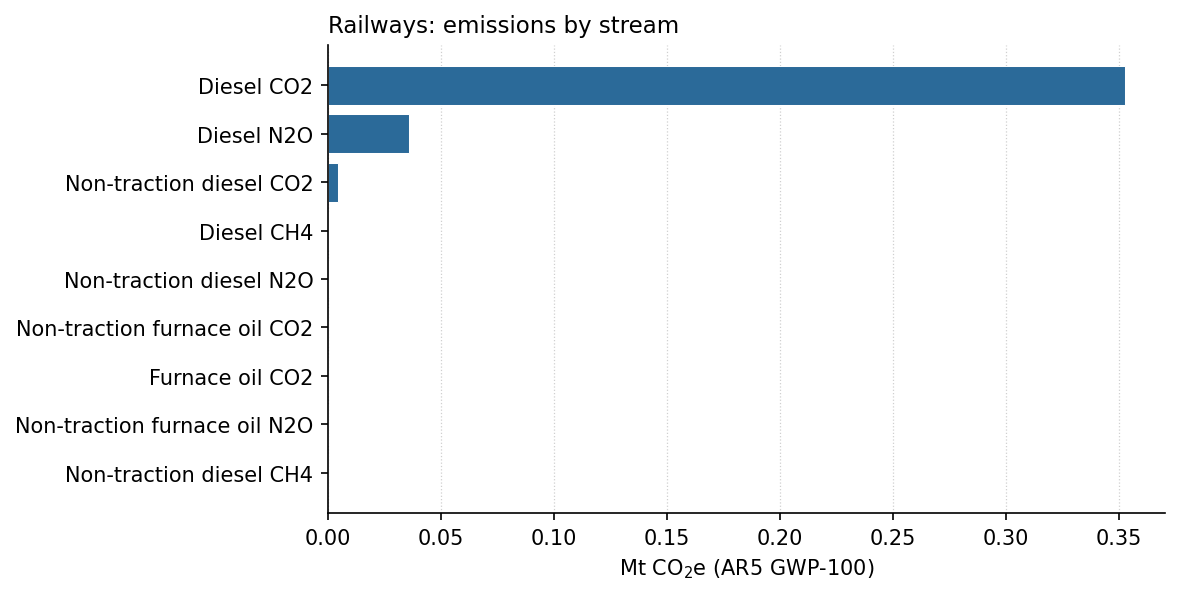
\includegraphics[width=\linewidth]{railways_streams.png}
\caption{Emissions by stream. \COtwo{} is \SI{90.6}{\percent} of the category and \NtwoO{} is
\SI{9.3}{\percent}, which is the entire reason the factor-table choice matters.}
\label{fig:streams}
\end{figure}

The uncertainty structure is unusual for this inventory. Diesel \COtwo{} at
$\pm\SI{5.4}{\percent}$ is the best-constrained stream in the whole national estimate---a
single state operator's metered consumption against a factor whose 95\% interval spans
\SI{3}{\percent}---while \NtwoO{} at $\pm\SI{150.1}{\percent}$ is among the worst. The sector
is simultaneously the most accurately measured and, in its second gas, the least confidently
factored.

\subsection{The factor-table diagnostic}

\begin{table}[htbp]
\centering
\footnotesize
\begin{tabular}{@{}lr@{}}
\toprule
\textbf{Case} & \textbf{Mt \COe{}} \\
\midrule
Rail table (3.4.1), reported     & 0.39437 \\
Road table (3.2.2) substituted   & 0.36282 \\
\bottomrule
\end{tabular}
\caption{What the sector would report on the road \NtwoO{} factor. The gap is
\SI{8.0}{\percent} of the category and \SI{100}{\percent} of the reason the table choice is
pinned by a test.}
\label{tab:diagnostic}
\end{table}

\subsection{The air-pollutant layer}

\begin{table}[htbp]
\centering
\footnotesize
\begin{tabular}{@{}lrr@{}}
\toprule
\textbf{Pollutant} & \textbf{kt, FY2023--24} & \textbf{$\pm$\%} \\
\midrule
NO\textsubscript{x} & 5.8749 & 65.2 \\
CO                  & 1.1996 & 61.2 \\
NMVOC               & 0.5213 & 65.2 \\
TSP                 & 0.1704 & 100.1 \\
PM\textsubscript{10}  & 0.1614 & 100.1 \\
PM\textsubscript{2.5} & 0.1536 & 100.1 \\
BC                  & 0.0998 & 104.4 \\
\SOtwo{}            & 0.1176 & 100.1 \\
NH\textsubscript{3} & 0.0008 & 57.2 \\
\bottomrule
\end{tabular}
\caption{Railway air pollutants, EMEP/EEA Tier~1 on the metered fuel; native mass, never
\COe{}. BC is a component of PM\textsubscript{2.5}; \SOtwo{} is the \SI{500}{ppm}
reference case of a \SIrange{0.008}{2.25}{\kilo\tonne} sulfur ladder.}
\label{tab:air}
\end{table}

\begin{figure}[htbp]
\centering
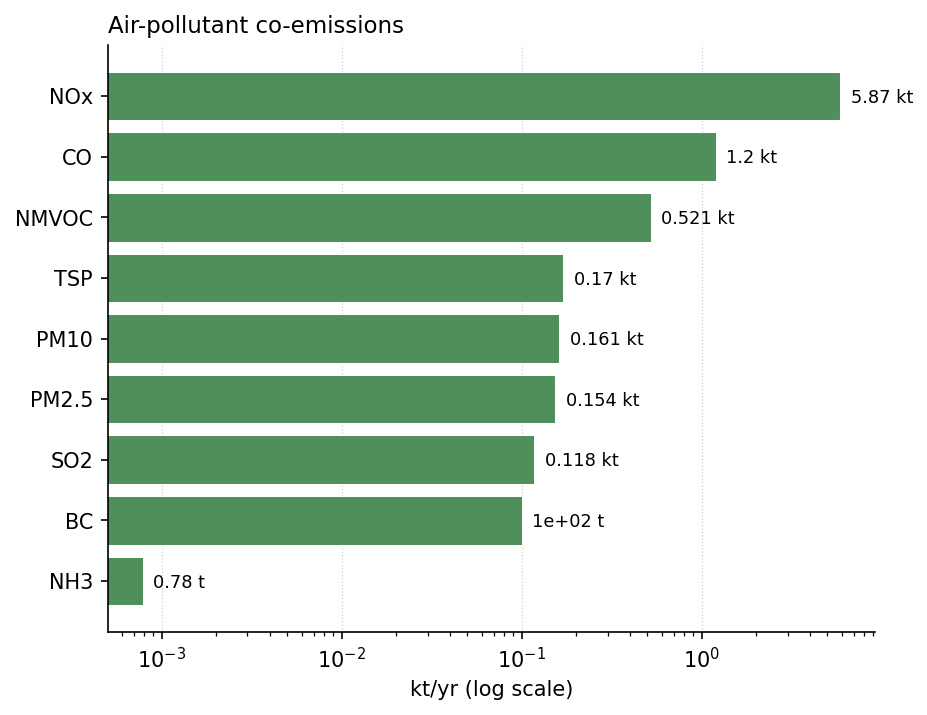
\includegraphics[width=\linewidth]{railways_air.png}
\caption{The air layer on a log axis: NO\textsubscript{x} in the kilotonnes, the
particulate family in the low hundreds of tonnes, black carbon just under \num{100}
tonnes.}
\label{fig:air}
\end{figure}

For scale: railway NO\textsubscript{x} at \SI{5.9}{\kilo\tonne} is a small national term,
but it is emitted in a hundred-metre-wide corridor through the centres of Pakistan's
largest cities, which is what the route-constrained surfaces of
Section~\ref{sec:spatial} exist to place. \SOtwo{} is the one pollutant whose national
value is genuinely open: on Euro-V fuel throughout it would be \SI{0.008}{\kilo\tonne}, on
the historical \SI{1}{\percent} specification \SI{2.25}{\kilo\tonne}---a \num{287}-fold
span that only an operator fuel-quality certificate can close.

\subsection{The series, and what it shows about Pakistani rail}

\begin{figure}[htbp]
\centering
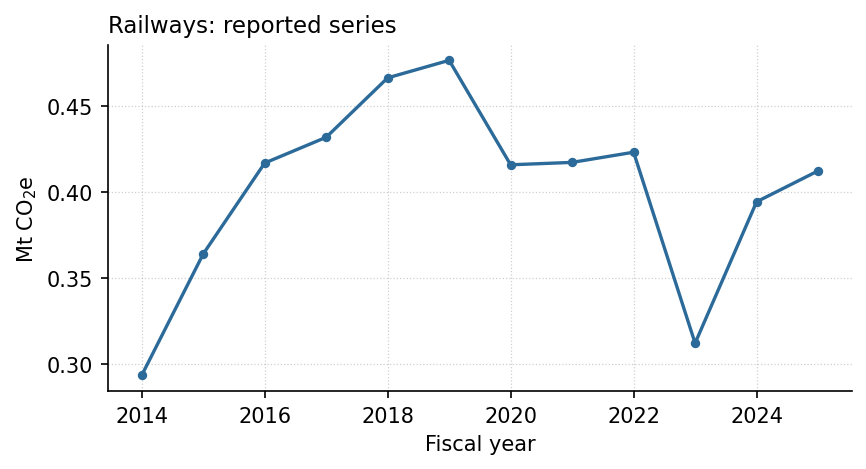
\includegraphics[width=\linewidth]{railways_timeseries.png}
\caption{FY2014--FY2025, unbroken. Emissions rise from \SI{0.294}{} to
\SI{0.412}{\mega\tonne} as diesel consumption rises from \num{98212} to \num{138673} thousand
litres, peaking at \SI{0.477}{\mega\tonne} in FY2019; the reference year FY2023--24 stands at
\SI{0.394}{\mega\tonne}. FY2018 and FY2019 were previously absent, recovered from the
2020--21 edition's historical table; FY2025 is provisional by its edition's own declaration.}
\label{fig:series}
\end{figure}

Three features, one of them only visible now the gaps are filled. The trend is upward---two
fifths more fuel across the twelve-year series, against a national inventory in which most
transport categories also grew. The series is volatile, dropping from \SI{0.423}{} in FY2022 to
\SI{0.312}{\mega\tonne} in FY2023 before recovering. And it peaks in FY2019 at
\SI{0.477}{\mega\tonne}, \SI{22}{\percent} above the reference year---a maximum that sat
inside the two recovered years and was therefore invisible in every previous version of this
figure. A single operator's annual fuel account is still a lumpy quantity, sensitive to
service suspensions, locomotive availability and the timing of procurement and depot issues,
and under the annual-equivalence assumption of Section~\ref{sec:data} the series should be
read as the operator's fuel account rather than as a smooth measure of traffic.

\subsection{Provincial allocation}

\begin{figure}[htbp]
\centering
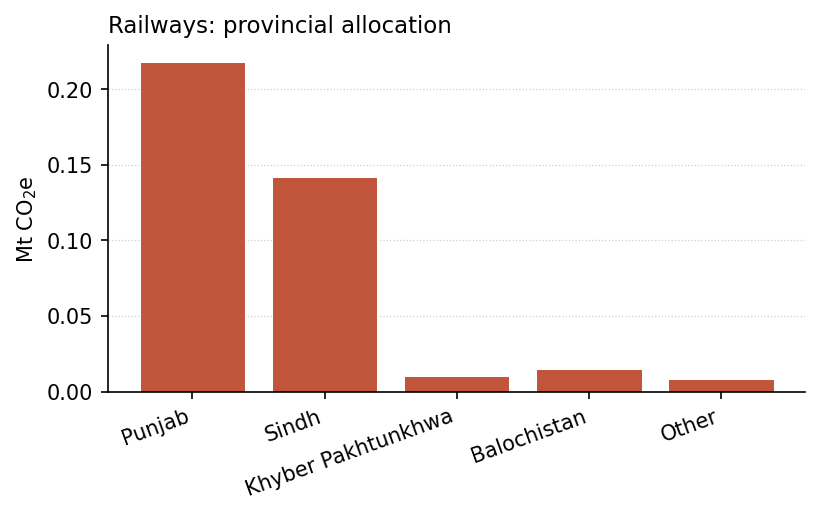
\includegraphics[width=\linewidth]{railways_provincial.png}
\caption{Punjab \SI{0.218}{\mega\tonne}, Sindh \SI{0.142}{\mega\tonne}, Balochistan
\SI{0.015}{\mega\tonne}, Khyber Pakhtunkhwa
\SI{0.010}{\mega\tonne}. Allocated on the route-constrained model of
Section~\ref{sec:spatial}; the residual share is the Islamabad Capital Territory trackage.}
\label{fig:provincial}
\end{figure}

The route model reverses the previous picture. The freight-wagons proxy put Sindh at
\SI{66}{\percent} because Karachi loads most wagons; constrained to the network that
actually burns the fuel, \SI{56}{\percent} of emissions land in Punjab, whose trunk
corridors carry the long-haul services both ways. The corridor weights beneath that split
are declared judgment pending the operator's timetable, so the wagons alternative is
retained as a structural scenario---Sindh \SI{66}{\percent} against \SI{36}{\percent}---and
the difference between the two is the honest statement of the split's uncertainty. What the
route model adds that no provincial proxy could: emissions sit on cells with track or
yards, nowhere else, which is the property an air-quality model actually needs.

\subsection{Place in the national inventory}

At \SI{0.09}{\percent} of the national total, railways is not a key category by level and
contributes nothing measurable to national variance. It is included because completeness is a
property of an inventory rather than of its largest categories, and because the attribution
it settles---national diesel the road category once absorbed wholesale, now excluded from the
road control at its source and verified by an independent two-source comparison---is roughly
a third of a megatonne, the size of this entire sector.
